\clearpage
\section{More experiments in LM pre-training}\label{appendix_model}

\subsection{Optimization} 

\textbf{Learning rate.} In Section~\ref{sec4}, we find that attention sink appears less obvious in LMs trained with small learning rates. This conclusion holds even if we compensate for more training steps. In our basic setup, we adopt a learning rate of 4e-4 for 20k training steps. When we scale the learning rate to half, i.e., 2e-4, we scale the training steps to 2 times, i.e., 40k.  As shown in Table~\ref{lr}, when we keep the multiply between learning rate and training steps constant (highlighted using cyan color), LMs trained with smaller learning rates tend to exhibit less obvious attention sink. Therefore, we conclude that small learning rates not only slow down the increase of attention sink but also mitigate attention sink even with longer training durations.\looseness=-1

\begin{table}[htbp]
\caption{Attention sink appears less obvious in LMs trained with small learning rates even compensating for more training steps.}
\vspace{-.2cm}
\begin{center}
\begin{tabular}{c|ccc}
\toprule
learning rate & training steps (k) & $\textrm{Sink}_1^{\epsilon}$(\%)  & valid loss \\
\midrule
\rowcolor{LightCyan}
8e-4 & 10 & 23.44 & 3.79 \\
8e-4 & 20 & 32.23  & 3.70 \\
\rowcolor{LightCyan}
4e-4 & 20 & 18.18 &  3.73 \\
2e-4 & 20 & 11.21 & 3.78 \\
\rowcolor{LightCyan}
2e-4 & 40 & 16.81 & 3.68 \\ 
1e-4 & 20 & \,\,\,2.90 & 3.92\\
\rowcolor{LightCyan}
1e-4 & 80 & \,\,\,6.29 & 3.67 \\
\bottomrule
\end{tabular}
\end{center}
\vspace{-.2cm}
\label{lr}
\end{table}

\textbf{Batch size.} During the pre-training, we consider different batch sizes with other hyper-parameters fixed. As shown in Table~\ref{batch_fix}(\emph{Left}), batch size does not affect the emergence of attention sink.




% \begin{table}[t]
% \vspace{-1.1cm}
% \caption{(\emph{Left}) With a smaller learning rate, attention sink tends to be less obvious. However, a much smaller learning rate leads to suboptimal optimization, thus no attention sink. (\emph{Right}) Batch size has no effect on the emergence of attention sink.\looseness=-1}
% \vspace{-.2cm}
% \begin{minipage}[t]{0.49\linewidth}
% \begin{center}
% \begin{tabular}{l|cccc}
% \toprule
% lr & 1e-3 & 4e-4 & 1e-4 & 1e-5 \\
% \midrule
% $\textrm{Sink}_1^{\epsilon}$(\%) & 33.04 & 18.18 & 4.13 & 0.19\\
% valid loss & \,\,\,3.69 & \,\,\,3.73 & 3.78 & 4.69  \\
% \bottomrule
% \end{tabular}
% \end{center}
% \end{minipage}
% \hfill
% \begin{minipage}[t]{0.49\linewidth}
% \begin{center}
% \begin{tabular}{l|cccc}
% \toprule
% batch size & 0.25M & 0.5M & 1M & 2M \\
% \midrule
% $\textrm{Sink}_1^{\epsilon}$(\%) & 16.45 & 17.19 & 18.18 & 16.19 \\
% valid loss & \,\,\,3.92 & \,\,\,3.78 & \,\,\,3.73 & \,\,\,3.68 \\
% \bottomrule
% \end{tabular}
% \end{center}
% \end{minipage}
% \vspace{-.2cm}
% \label{lr_batch}
% \end{table}

\subsection{Data distribution} 

\textbf{Training data amount.} In Section~\ref{sec5}, we find that with less training data, attention sink also disappears. Meanwhile, LMs are also prone for overfitting. To disentangle the effects of training data amount and overfitting on attention sink, we monitor the dynamics of train/valid loss and attention sink metric during the LM pre-training in a more granular level, as present in Figure~\ref{appendix_overfit}.  With only 50M and 100M training data, LMs overfit at very early stages, between 1k and 2k steps. Meanwhile, $\textrm{Sink}_1^{\epsilon}$ maintains a very small value (less than 1\%). While for the setup of 5B training data, $\textrm{Sink}_1^{\epsilon}$ keeps increasing after a certain step. This indicates that the amount of training data, instead of overfitting, plays an important role in the emergence of attention sink.\looseness=-1


\begin{figure}[htbp]
\centering
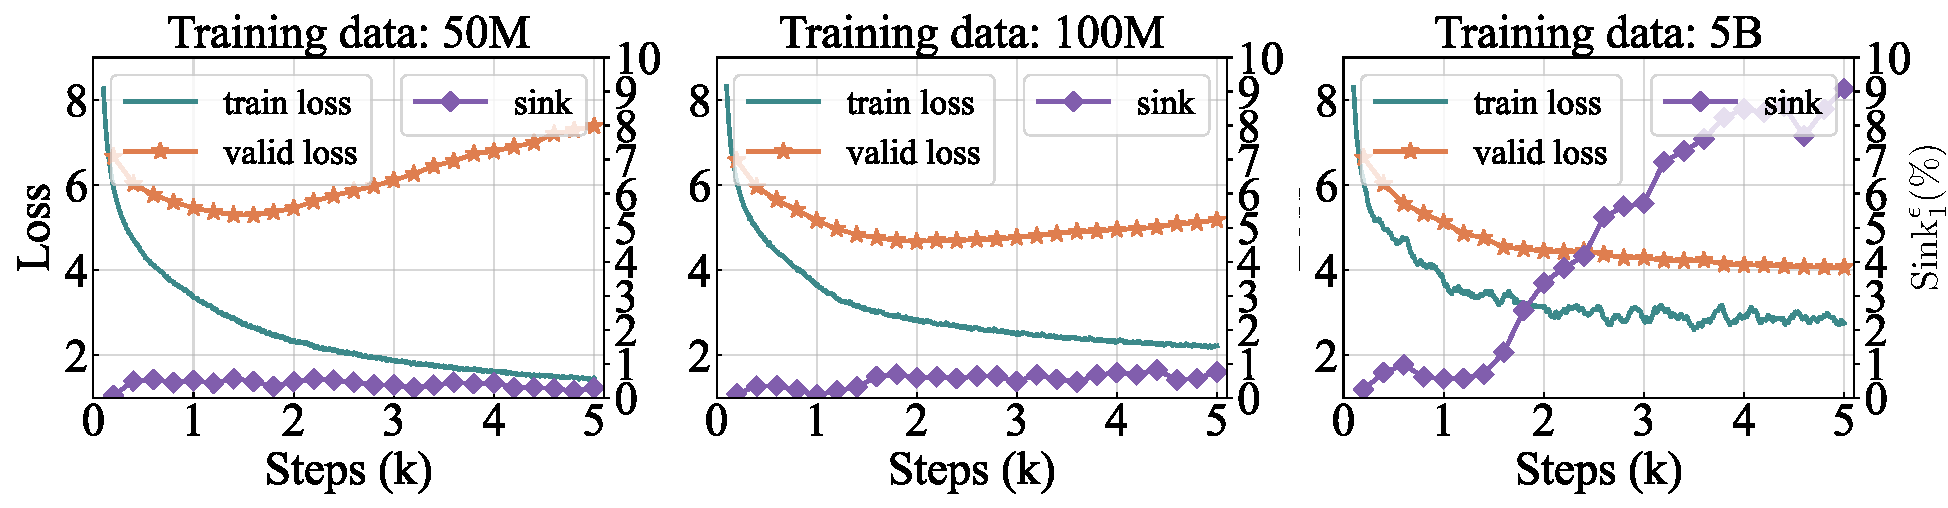
\includegraphics[width=\textwidth]{figures/overfit.pdf}
% \vspace{-0.85cm}
\caption{Dynamics of train/valid loss and $\textrm{Sink}_1^{\epsilon}$ during LM pre-training under different amounts of training data: (\emph{Left}) 50M; (\emph{Middle}) 100M; (\emph{Right}) 5B.\looseness=-1}
\label{appendix_overfit}
\end{figure}


\textbf{Fixing token in a specific position.} During the pre-training, we consider fixing the token $\boldsymbol{x}_{\textrm{fix}}$ in the first/second/third position. Consequently, when evaluating the attention sink metric, in Table~\ref{batch_fix}(\emph{Right}), we find that attention sink appears in the appears in the fixed token instead of the first token.\looseness=-1

\begin{table}[htbp]
% \vspace{-1.1cm}
\caption{(\emph{Left}) Batch size has no effect on the emergence of attention sink. (\emph{Right}) Attention sink appears in the appears in the fixed token instead of the first token.\looseness=-1}
\begin{minipage}[t]{0.52\linewidth}
\begin{center}
\begin{tabular}[t]{l|cccc}
\toprule
Batch size & 0.25M & 0.5M & 1M & 2M \\
\midrule
$\textrm{Sink}_1^{\epsilon}$(\%) & 16.45 & 17.19 & 18.18 & 16.19 \\
valid loss & \,\,\,3.92 & \,\,\,3.78 & \,\,\,3.73 & \,\,\,3.68 \\
\bottomrule
\end{tabular}
\end{center}
\end{minipage}
\hfill
\begin{minipage}[t]{0.47\linewidth}
\begin{center}
\begin{tabular}[t]{l|cccc}
\toprule  %$\boldsymbol{x}_1=\boldsymbol{x}_{\textrm{fix}}$
Fixed position & 1 & 2 & 3 \\
\midrule
$\textrm{Sink}_1^\epsilon$ (\%) & 74.11 & \,\,\,0.00 & \,\,\,0.00 \\
$\textrm{Sink}_2^\epsilon$ (\%) & \,\,\,0.00 & 69.03 & \,\,\,0.00 \\
$\textrm{Sink}_3^\epsilon$ (\%) & \,\,\,0.00 & \,\,\,0.00 & 69.64 \\
$\textrm{Sink}_4^\epsilon$ (\%) & \,\,\,0.01 & \,\,\,0.01 & \,\,\,0.00 \\
% % \midrule
% $\beta_1$ & 3.18 & 3.16 & 3.38 & 3.27 \\
\bottomrule
\end{tabular}
\end{center}
\end{minipage}
% \vspace{-.2cm}
\label{batch_fix}
\end{table}

% \begin{table}[htbp]
% \caption{Attention sink appears in the appears in the fixed token instead of the first token.}
% \vspace{-.2cm}
% \begin{center}
% \begin{tabular}{l|cccc}
% \toprule  %$\boldsymbol{x}_1=\boldsymbol{x}_{\textrm{fix}}$
% Fixed position & 1 & 2 & 3 \\
% \midrule
% $\textrm{Sink}_1^\epsilon$ (\%) & 74.11 & \,\,\,0.00 & \,\,\,0.00 \\
% $\textrm{Sink}_2^\epsilon$ (\%) & \,\,\,0.00 & 69.03 & \,\,\,0.00 \\
% $\textrm{Sink}_3^\epsilon$ (\%) & \,\,\,0.00 & \,\,\,0.00 & 69.64 \\
% $\textrm{Sink}_4^\epsilon$ (\%) & \,\,\,0.01 & \,\,\,0.01 & \,\,\,0.00 \\
% % % \midrule
% % $\beta_1$ & 3.18 & 3.16 & 3.38 & 3.27 \\
% \bottomrule
% \end{tabular}
% \end{center}
% \vspace{-.2cm}
% \label{fix_token}
% \end{table}


\subsection{FFN design} 

\textbf{Activation functions.} Since FFN in the earlier transformer block blasts off the $\ell_2$-norm of the first token, we are wondering whether the choices of activation functions in FFN will affect the attention sink. Besides the SwiGLU activations used in our default setup, we also consider other activation functions, as present in Table~\ref{activation}. We observe that different FFN designs do not affect the emergence of attention sink.\looseness=-1


\begin{table}[htbp]
\caption{Modifying the activation functions in FFN does not affect the emergence of attention sink.}
\vspace{-.2cm}
\begin{center}
\begin{tabular}{l|lccc}
\toprule
Activation functions & $\boldsymbol{F}$ & $\textrm{Sink}_1^{\epsilon}$(\%)  & valid loss \\
\midrule
ReLU & $\textrm{ReLU}(\boldsymbol{h}\boldsymbol{W}_1)\boldsymbol{W}_2$ & 16.90 &  3.82\\
GeLU~\citep{hendrycks2016gaussian} & $\textrm{GeLU}(\boldsymbol{h}\boldsymbol{W}_1)\boldsymbol{W}_2$ & 14.76   &  3.79 \\
Swish~\citep{ramachandran2017searching} & $\textrm{Swish}(\boldsymbol{h}\boldsymbol{W}_1)\boldsymbol{W}_2$ &  17.89 & 3.80 \\
ReGLU~\citep{shazeer2020glu} & $\left(\textrm{ReLU}(\boldsymbol{h}\boldsymbol{W}_1)\odot\boldsymbol{h}\boldsymbol{W}_2\right)\boldsymbol{W}_3$ & 13.88  & 3.75\\
GeGLU~\citep{shazeer2020glu} & $\left(\textrm{GeLU}(\boldsymbol{h}\boldsymbol{W}_1)\odot\boldsymbol{h}\boldsymbol{W}_2\right)\boldsymbol{W}_3$ &  17.86 & 3.73\\
SwiGLU~\citep{shazeer2020glu} & $\left(\textrm{Swish}(\boldsymbol{h}\boldsymbol{W}_1)\odot\boldsymbol{h}\boldsymbol{W}_2\right)\boldsymbol{W}_3$ &  18.18 & 3.73\\
\bottomrule
\end{tabular}
\end{center}
\vspace{-.2cm}
\label{activation}
\end{table}

\subsection{Attention design}

\textbf{Multi-head design in attention.} We consider two perspectives in multi-head design in attention. Firstly, we explore whether the number of heads has an impact on attention sink, especially for $H=\textrm{1}$, which refers to single-head self-attention. Second, attention output from each head is concatenated: $\boldsymbol{O}^l=\textrm{Concat}_{h=1}^H\left(\boldsymbol{A}^{l\textrm{,}h}\boldsymbol{V}^{l\textrm{,}h}\right)\boldsymbol{W}_{O}^l$. We replace such concatenation operation with addition operation: $\boldsymbol{O}^l=\sum_{h=1}^H\left(\boldsymbol{A}^{l\textrm{,}h}\boldsymbol{V}^{l\textrm{,}h}\right)\boldsymbol{W}_{O}^l$. As shown in Table~\ref{multi_head}(\emph{Left}), multi-head design does not affect the emergence of attention sink.

\begin{table}[htbp]
\caption{(\emph{Left}) Modifying multi-head design does not affect the emergence of attention sink. (\emph{Right}) Sharing KV biases across heads in each block results in attention sink shifting back to the first token from K biases.}
% \vspace{-.2cm}
\begin{minipage}[t]{0.4\linewidth}
\begin{center}
\begin{tabular}[t]{l|cc}
\toprule
Multi-head & $\textrm{Sink}_1^{\epsilon}$ (\%) & valid loss \\
\midrule
$H=\textrm{8}$ & 18.18 & 3.73\\
$H=\textrm{4}$ & 10.68 & 3.74\\
$H=\textrm{2}$ & 12.95 & 3.76\\
$H=\textrm{1}$ & 19.50 & 3.78\\
addition & 21.76 & 3.74\\
\bottomrule
\end{tabular}
\end{center}
\end{minipage}
\hfill
\begin{minipage}[t]{0.58\linewidth}
\begin{center}
\begin{tabular}[t]{l|cccc}
\toprule
Head-sharing & $\checkmark$ & $\checkmark$  & $\times$ & $\times$ \\
Biases type & KV & KV & K & K \\
\midrule
$\textrm{Sink}_{*}^{\epsilon}$(\%)  & 72.76 & 56.61 & 73.34 & 68.31  \\
$\textrm{Sink}_1^{\epsilon}$(\%) &   \,\,\,0.04 & 12.44 & \,\,\,0.00 & \,\,\,0.23 \\
valid loss & \,\,\,3.72 & \,\,\,3.72 & \,\,\,3.72 & \,\,\,3.72\\
\bottomrule
\end{tabular}
\end{center}
\end{minipage}
% \vspace{-.2cm}
\label{multi_head}
\end{table}

% \begin{table}[htbp]
% \caption{Sharing KV biases across heads in each block results in attention sink shifting back to the first token from K biases.}
% \vspace{-.2cm}
% \begin{center}
% \begin{tabular}{l|cccc}
% \toprule
% Head-sharing & $\checkmark$ & $\checkmark$  & $\times$ & $\times$ \\
% Biases type & KV & KV & K & K \\
% \midrule
% $\textrm{Sink}_{*}^{\epsilon}$(\%)  & 72.76 & 56.61 & 73.34 & 68.31  \\
% $\textrm{Sink}_1^{\epsilon}$(\%) &   0.04 & 12.44 & 0.00 & 0.23 \\
% valid loss & 3.72 & 3.72 & 3.72 & 3.72\\
% \bottomrule
% \end{tabular}
% \end{center}
% \vspace{-.2cm}
% \label{head_share}
% \end{table}


% \begin{table}[htbp]
% \caption{Modifying multi-head design does not affect the emergence of attention sink.}
% % \vspace{-.2cm}
% \begin{minipage}[t]{0.52\linewidth}
% \begin{center}
% \begin{tabular}{l|ccccc}
% \toprule
% Multi-head & $H=\textrm{8}$  & $H=\textrm{4}$ & $H=\textrm{2}$ & $H=\textrm{1}$ & multi-head addition\\
% \midrule
% $\textrm{Sink}_1^{\epsilon}$ (\%) & 18.18 & 10.68 & 12.95 & 19.50 & 21.76 \\
% % \midrule
% valid loss & \,\,\,3.73  & \,\,\,3.74 & \,\,\,3.76 & \,\,\,3.78 &  \,\,\,3.74 \\
% \bottomrule
% \end{tabular}
% \end{center}
% \end{minipage}
% \hfill
% \begin{minipage}[t]{0.52\linewidth}
% \end{minipage}
% % \vspace{-.2cm}
% \label{multi_head}
% \end{table}

\textbf{Head-sharing K/KV biases in attention.} In the main paper, we consider both KV biases and V biases in attention. These biases are not shared by different heads in each block. We further explore whether head-sharing patterns will affect their functionality. As present in Table~\ref{multi_head}(\emph{Right}), LMs with KV biases are more likely affected by the head-sharing pattern: attention sink shifts from the K biases to the first token. While LMs with K biases are less affected. 

\begin{table}[htbp]
\vspace{-0.2cm}
\caption{Even with very few learnable dimensions for $\boldsymbol{k}^{*l\textrm{,}h}$, large attention appears in $\boldsymbol{k}^{*l\textrm{,}h}$.\looseness=-1}
\vspace{-.4cm}
\begin{center}
\begin{tabular}{l|ccccccc}
\toprule
$d_a$ & 1 & 2 & 4 & 8 & 16 & 32  & 64  \\
\midrule
$\textrm{Sink}_{*}^{\epsilon}$(\%) & 32.18 & 30.88 & 30.94 & 31.39 & 23.30 & 51.23 &  69.19 \\
$\textrm{Sink}_{1}^{\epsilon}$(\%) & \,\,\,4.74 &  \,\,\,4.96 & \,\,\,4.39 & \,\,\,4.54 & \,\,\,2.19 & \,\,\,1.94 & \,\,\,0.04 \\
valid loss & \,\,\,3.73 & \,\,\,3.72 & \,\,\,3.72 & \,\,\,3.73 & \,\,\,3.73 & \,\,\,3.73 & \,\,\,3.72 \\
\bottomrule
\end{tabular}
\end{center}
\vspace{-.4cm}
\label{k_low_rank}
\end{table}

\textbf{Learnable dimensions of K biases.} In the setup of K biases, we set all dimensions of $\boldsymbol{k}^{*l\textrm{,}\,h}$ as learnable weights. In Section~\ref{section3_1}, we have shown that K biases are distributed in a different manifold, with low rank. Therefore, we consider only $d_a$ dimensions of $\boldsymbol{k}^{*l\textrm{,}\,h}$ are adjustable/learnable while the other $d_h-d_a$ dimensions are zeros. As present in Table~\ref{k_low_rank}, with very few learnable dimensions, even for $d_a=\textrm{1}$, $\boldsymbol{k}^{*l\textrm{,}\,h}$ are still allocated significant attention. With more learnable dimensions, the attention sink appears more obvious. 

\textbf{Scaling the normalization in softmax attention.} Before our experiments about replacing softmax attention, we first explore the effects of normalization scales in softmax attention. In the main paper, the attention output for the $i$-th output is
\begin{equation}
\boldsymbol{v}_i^{\dagger}=\sum_{j=1}^i\frac{\textrm{sim}(\varphi(\boldsymbol{q}_i)\textrm{,}\,\varphi(\boldsymbol{k}_j))}{\sum_{j'=1}^i\textrm{sim}(\varphi(\boldsymbol{q}_i)\textrm{,}\,\varphi(\boldsymbol{k}_{j'}))}\boldsymbol{v}_j=\sum_{j=1}^i\frac{\textrm{sim}(\varphi(\boldsymbol{q}_i)\textrm{,}\,\varphi(\boldsymbol{k}_j))}{\boldsymbol{Z}_i}\boldsymbol{v}_j\textrm{.}
\end{equation}

We consider a scale factor $\alpha$, the normalization term is $\boldsymbol{Z}_i=\frac{1}{\alpha}\sum_{j'=1}^i\textrm{sim}(\varphi(\boldsymbol{q}_i)\textrm{,}\,\varphi(\boldsymbol{k}_j))$, and then the attention score are sum up to $\alpha$. For default setup, $\alpha=\textrm{1}$. As shown in Table~\ref{reweight}(\emph{Left}), with a smaller normalization scale, attention sink tends to appear in fewer heads. From another perspective,
\begin{equation}
\boldsymbol{v}_i^{\dagger}=\sum_{j=1}^i\frac{\alpha
\textrm{sim}(\varphi(\boldsymbol{q}_i)\textrm{,}\,\varphi(\boldsymbol{k}_j))}{\sum_{j'=1}^i\textrm{sim}(\varphi(\boldsymbol{q}_i)\textrm{,}\,\varphi(\boldsymbol{k}_{j'}))}\boldsymbol{v}_j=\sum_{j=1}^i\frac{
\textrm{sim}(\varphi(\boldsymbol{q}_i)\textrm{,}\,\varphi(\boldsymbol{k}_j))}{\sum_{j'=1}^i\textrm{sim}(\varphi(\boldsymbol{q}_i)\textrm{,}\,\varphi(\boldsymbol{k}_{j'}))}\boldsymbol{h}_j(\alpha\boldsymbol{W}_V)\textrm{,}
\end{equation}
\begin{equation}
    \boldsymbol{o}_i'=\textrm{Concat}_{h=1}^H (\boldsymbol{v}_i^{'h})\boldsymbol{W}_O\textrm{.}
\end{equation}

Therefore, this normalization scale can be regarded as the scale for $\boldsymbol{W}_V$ or $\boldsymbol{W}_O$. We show that this normalization scaling could be implemented by scaling learning rates and initialization. We use the $s$ to represent the optimization step, and $s=\textrm{0}$ refers to the initialization. When scaling the normalization, we have the following SGD update rule (take $\boldsymbol{W}_O$ for example):
\begin{align}
    \boldsymbol{W}_O^{s+1}&=\boldsymbol{W}_O^{s}-\eta\nabla_{\boldsymbol{W}_O^{s}} \mathcal{L}(\alpha\boldsymbol{W}_O^{s})\\
    &=\boldsymbol{W}_O^{s}-\alpha\eta\nabla_{\boldsymbol{W}} \mathcal{L}(\boldsymbol{W})|_{\boldsymbol{W}=\alpha\boldsymbol{W}_O^{s}}\textrm{,}
\end{align}
where $\eta$ is the original learning rate. Suppose we only modify the learning rate and initialization, to ensure each optimization step $\hat{\boldsymbol{W}}_O^{s}=\alpha\boldsymbol{W}_O^{s}$, we need first to ensure $\hat{\boldsymbol{W}}_O^{0}=\alpha\boldsymbol{W}_O^{0}$. Suppose that we have $\hat{\boldsymbol{W}}_O^{s}=\boldsymbol{W}_O^{s}$, then the update rule is:
\begin{align}
\hat{\boldsymbol{W}}_O^{s+1}&=\hat{\boldsymbol{W}}_O^{s}-\eta'\nabla_{\hat{\boldsymbol{W}}_O^{s}} \mathcal{L}(\hat{\boldsymbol{W}}_O^{s})\\
&=\alpha\boldsymbol{W}_O^{s}-\eta'\nabla_{\boldsymbol{W}} \mathcal{L}(\boldsymbol{W})|_{\boldsymbol{W}=\alpha\boldsymbol{W}_O^{s}}\textrm{,}
\end{align}

 To ensure $\hat{\boldsymbol{W}}_O^{s+1}=\alpha\boldsymbol{W}_O^{s+1}$, we need the new learning rate $\eta'$ meets $\eta'=\alpha^2\eta$. For advanced optimization algorithms, e.g., Adam~\citep{kingma2014adam} and AdamW~\citep{loshchilov2017decoupled}. We have the following update rule (take AdamW for example, $\gamma$ refers to the weight decay ratio): 
 \begin{align}
\boldsymbol{g}_{s+1} &= \nabla_{\boldsymbol{W}_O^{s}} \mathcal{L}(\alpha\boldsymbol{W}_O^{s}) = \alpha\nabla_{\boldsymbol{W}} \mathcal{L}(\boldsymbol{W})|_{\boldsymbol{W}=\alpha\boldsymbol{W}_O^{s}} \\
\boldsymbol{m}_{s+1} &= \beta_1\boldsymbol{m}_{s} + (1-\beta_1)\boldsymbol{g}_{s+1} \\
\boldsymbol{v}_{s+1} &= \beta_2\boldsymbol{v}_{s} + (1-\beta_2)\boldsymbol{g}^2_{s+1} \\
\boldsymbol{W}_O^{s+1}&=(1-\eta\gamma) \boldsymbol{W}_O^{s} - \eta \frac{\boldsymbol{m}_{s+1} / (1 - \beta_1^t)}{\sqrt{\boldsymbol{v}_{s+1}/ (1-\beta_2^t)} + \epsilon}
\end{align}

We denote $\hat{\boldsymbol{g}}_{s+1},\,\hat{\boldsymbol{m}}_{s+1},\,\hat{\boldsymbol{v}}_{s+1}$ represents the intermediate counterparts for update of scenario where we only modify learning rate and initialization. First, we also need to ensure the initialization $\hat{\boldsymbol{W}}_O^{0}=\alpha\boldsymbol{W}_O^{0}$. Then we assume that we have already matched $\hat{\boldsymbol{W}}_O^{s}=\alpha\boldsymbol{W}_O^{s}$. The gradient for each step is\looseness=-1
\begin{equation}
    \hat{\boldsymbol{g}}_{s+1} = \nabla_{\hat{\boldsymbol{W}}_O^{s}} \mathcal{L}(\hat{\boldsymbol{W}}_O^{s}) = \nabla_{\boldsymbol{W}} \mathcal{L}(\boldsymbol{W})|_{\boldsymbol{W}=\alpha\boldsymbol{W}_O^{s}}= \boldsymbol{g}_{s+1} / \alpha
\end{equation}

Then the first and second moment will be $\hat{\boldsymbol{m}}_{s+1}=\boldsymbol{m}_{s+1} / \alpha$ and  $\hat{\boldsymbol{v}}_{s+1}=\boldsymbol{v}_{s+1} / \alpha^2$. The updated weights will be 
\begin{align}
\hat{\boldsymbol{W}}_O^{s+1}&=(1-\eta'\gamma') \hat{\boldsymbol{W}}_O^{s} - \eta' \frac{\hat{\boldsymbol{m}}_{s+1} / (1 - \beta_1^t)}{\sqrt{\hat{\boldsymbol{v}}_{s+1}/ (1-\beta_2^t)} + \epsilon'}\\    
&=(1-\eta'\gamma') \alpha\boldsymbol{W}_O^{s} - \eta' \frac{\boldsymbol{m}_{s+1} /\alpha(1 - \beta_1^t)}{\sqrt{\boldsymbol{v}_{s+1}/ \alpha^2(1-\beta_2^t)} + \epsilon'} 
\end{align}

Therefore, to ensure $\hat{\boldsymbol{W}}_O^{s+1}=\alpha\boldsymbol{W}_O^{s+1}$, one solution is $\eta'=\alpha\eta$ and $\epsilon'=\epsilon / \alpha$ and $\gamma'=\gamma / \alpha$.


% We note that only if we assume that $\sqrt{\boldsymbol{v}_{s+1}/ (1-\beta_2^t)} \gg \epsilon$, we could ensure $\hat{\boldsymbol{W}}_O^{s}=\alpha\boldsymbol{W}_O^{s}$.

% \boldsymbol{W}_O^{s+1}&=\boldsymbol{W}_O^{s}-\eta\nabla \mathcal{L}(\alpha\boldsymbol{W}_O^{s})\\
    % &=\boldsymbol{W}_O^{s}-\alpha\eta\nabla \mathcal{L}(\boldsymbol{W})|_{\boldsymbol{W}=\alpha\boldsymbol{W}_O^{s}}\textrm{,}



\begin{table}[htbp]
\caption{(\emph{Left}) Scaling the normalization in Softmax attention to less than one can mitigate attention sink but not prevent its emergence. (\emph{Right}) LMs with sigmoid attention (without sigmoid attention) trained by different learning rates and weight decay ratios have no attention sink.}
% \vspace{-.2cm}
\begin{minipage}[t]{0.38\linewidth}
\begin{center}
\begin{tabular}[t]{c|cc}
\toprule
Scale $\alpha$ &$\textrm{Sink}_1^{\epsilon}$(\%) & valid loss\\
\midrule
2.0 & 29.10 & 3.72\\
1.0 & 18.18 & 3.73\\
0.2 & \,\,\,9.41 & 3.72\\
0.1 & \,\,\,3.59 & 3.76\\
0.05\,\,\, & \,\,\,4.53 & 3.78 \\
\bottomrule
\end{tabular}
\end{center}
% \vspace{-.2cm}
\end{minipage}
\hfill
\begin{minipage}[t]{0.60\linewidth}
\begin{center}
\begin{tabular}[t]{cc|cc}
\toprule
Learning rate & Weight decay & $\textrm{Sink}_1^{\epsilon}$(\%) & valid loss \\
\midrule
4e-4 & 0.0 & 0.64 & 3.77 \\
4e-4 & 0.1 & 0.44 & 3.70 \\
4e-4 & 0.5 & 0.18 & 3.76 \\
4e-4 & 1.0 & 0.30 & 4.06 \\
1e-3 & 0.1 & 0.81 & 3.68 \\
1e-4 & 0.1 & 0.36 & 4.08\\
\bottomrule
\end{tabular}
\end{center}
\end{minipage}
\label{reweight}
\end{table}

% \begin{table}[htbp]
% \caption{LMs with sigmoid attention (without sigmoid attention) trained by different learning rates and weight decay ratios have no attention sink.}
% \vspace{-.2cm}
% \begin{center}
% \begin{tabular}{l|cccccc}
% \toprule
% Learning rate & 4e-4 & 4e-4 & 4e-4 & 4e-4 & 1e-3 & 1e-4\\
% Weight decay & 0.0 &  0.1 & 0.5 & 1.0 & 0.1 & 0.1 \\
% \midrule
% $\textrm{Sink}_1^{\epsilon}$(\%) & 0.64 & 0.44 & 0.18 & 0.30 & 0.81 & 0.36\\
% valid loss & 3.77 & 3.70 & 3.76 & 4.06 & 3.68 & 4.08  \\
% \bottomrule
% \end{tabular}
% \end{center}
% \vspace{-.2cm}
% \label{sigmoid}
% \end{table}

% $\alpha$ & 2.0 & 1.0 & 0.2 & 0.1 & 0.02 \\
% \midrule
% $\textrm{Sink}_1^{\epsilon}$(\%) & 29.10 & 18.18 & 9.41 & 3.59 & 4.53\\
% valid loss & 3.72 &  3.73 & 3.72 & 3.76 & 3.78  \\


\textbf{Normalizer.} Besides the normalizer $\boldsymbol{Z}_i=\sum_{j'=1}^i\textrm{sim}(\varphi(\boldsymbol{q}_i)\textrm{,}\,\varphi(\boldsymbol{k}_{j'}))$ considered in the main paper, we consider alternative normalizer: $\boldsymbol{Z}_i=\left(\sum_{j'=1}^i\textrm{sim}(\varphi(\boldsymbol{q}_i)\textrm{,}\,\varphi(\boldsymbol{k}_{j'}))^p\right)^{\frac{1}{p}}$, which gives us following attention operation: 
\begin{equation}
\boldsymbol{v}_i^{\dagger}=\frac{\sum_{j=1}^i\textrm{sim}(\varphi(\boldsymbol{q}_i)\textrm{,}\,\varphi(\boldsymbol{k}_j))\boldsymbol{v}_j}{\boldsymbol{Z}_i}=\frac{\sum_{j=1}^i\textrm{sim}(\varphi(\boldsymbol{q}_i)\textrm{,}\,\varphi(\boldsymbol{k}_j))\boldsymbol{v}_j}{\left(\sum_{j'=1}^i\textrm{sim}(\varphi(\boldsymbol{q}_i)\textrm{,}\,\varphi(\boldsymbol{k}_{j'}))^p\right)^{\frac{1}{p}}}\textrm{.}
\end{equation}


For softmax attention, we have $\textrm{sim}(\varphi(\boldsymbol{q}_i)\textrm{,}\,\varphi(\boldsymbol{k}_j))=\textrm{exp}(\frac{\boldsymbol{q}_i\boldsymbol{k}_j^\top}{\sqrt{d_h}})$, then we can derive that
\begin{equation}
    \boldsymbol{v}_i^{\dagger}=\frac{\sum_{j=1}^i\textrm{exp}(\frac{\boldsymbol{q}_i\boldsymbol{k}_j^\top}{\sqrt{d_h}}))\boldsymbol{v}_j}{\left(\sum_{j'=1}^i\textrm{exp}(\frac{\boldsymbol{q}_i\boldsymbol{k}_{j'}^\top}{\sqrt{d_h}})^p\right)^{\frac{1}{p}}}=\sum_{j=1}^i \left(\frac{\textrm{exp}(\frac{\boldsymbol{q}_i\boldsymbol{k}_j^\top}{\sqrt{d_h}/p})}{\sum_{j'=1}^i\textrm{exp}(\frac{\boldsymbol{q}_i\boldsymbol{k}_{j'}^\top}{\sqrt{d_h}/p})}\right)^{\frac{1}{p}}\boldsymbol{v}_j\textrm{.}
\end{equation}

This is equivalent to adding a temperature $1/p$ into the softmax attention logits, and then taking the $p$-root of attention scores after softmax. We call this $p$-normalized softmax attention. $p=\textrm{1}$ in regular softmax attention. Similarly, we construct the LMs with $p$-normalized sigmoid attention. 

We find that when $p=2$ or $p=3$ or $p=4$, pre-training of $p$-normalized softmax attention diverges and the loss goes infinity. When $p=1/2$ or $p=1/3$ or $p=1/4$, LM pre-training converges. As the attention scores are not added up to one, we investigate the massive activations instead, as visualized in Figure~\ref{appendix_normalizer}(\emph{Left}). With smaller $p$, massive activations are mitigated to some extent, but not as effective as sigmoid attention without normalization. Intuitively, smaller $p$ induces a larger temperature in softmax operation, which leads to flattened attention logits. 

Afterward, we conduct experiments on $p$-normalized sigmoid attention. There is no training problem with $p$ larger than 1. As visualized in Figure~\ref{appendix_normalizer}(\emph{Right}), LMs with $p$-normalized sigmoid attention still demonstrate strong massive activations. To conclude, different normalizers may affect the amplitude of attention sink, but not stop its emergence. 



\begin{figure}[htbp]
\centering
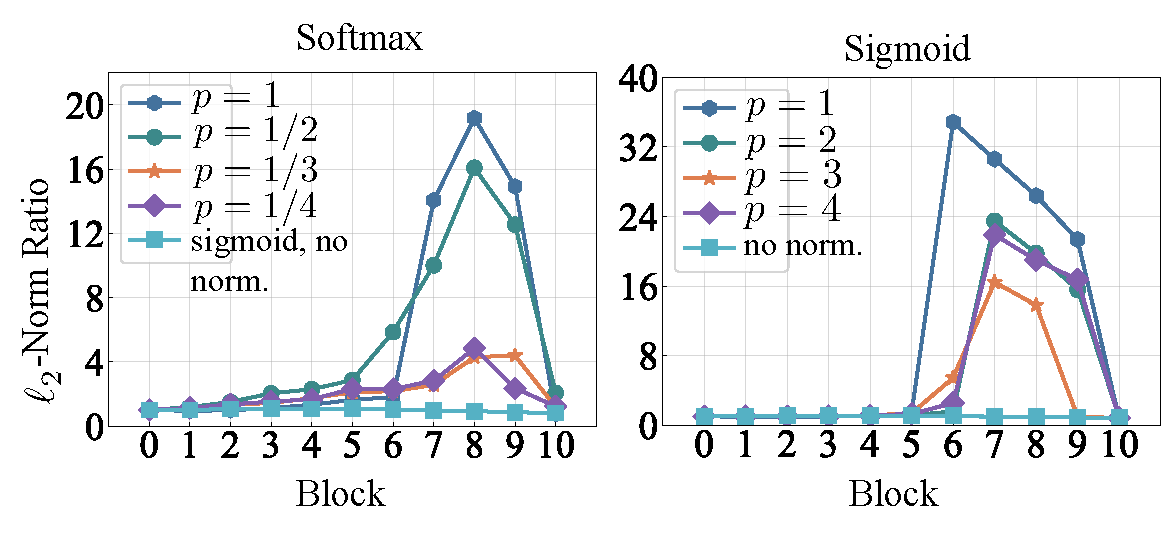
\includegraphics[width=0.7\textwidth]{figures/normalizer.pdf}
% \vspace{-0.85cm}
\caption{$\ell_2$-norm ratio of $\boldsymbol{h}_1^l$ and mean of $\boldsymbol{h}_{t\neq 0}^l$. (\emph{Left}) $p$-normalized softmax attention and also sigmoid attention without normalization (as reference). (\emph{Right}) $p$-normalized sigmoid attention and also sigmoid attention without normalization (as reference).\looseness=-1}
\label{appendix_normalizer}
\end{figure}

\textbf{Attention operations.} Firstly, we present all attempted attention operations in Table~\ref{appendix_operation}. It is noted that several setups lead to training failure. For LMs with sigmoid attention without normalization, we vary the learning rates or weight decay ratios $\gamma$. Consequently, as shown in Table~\ref{reweight}(\emph{Right}), the trained LMs still have no attention sink, which further confirms our conclusion in the main paper.



\begin{table}[htbp]
% \vspace{-1.cm}
\caption{Normalization and selections of kernels in attention significantly affect the emergence of the attention sink. We use ``*'' to mark that the metric $\textrm{Sink}_1^{\epsilon}$ is computed by proxy attention scores. We use ``-'' to represent the training failure under the setup.}
\vspace{-.2cm}
\begin{center}
\begin{tabular}{l|l|cc}
\toprule
  $\textrm{sim}(\varphi(\boldsymbol{q}_i)\textrm{,}\,\varphi(\boldsymbol{k}_j))$ & $\boldsymbol{Z}_i$ & $\textrm{Sink}_1^{\epsilon}$(\%) & valid loss \\
\midrule
 $\textrm{exp}(\frac{\boldsymbol{q}_i\boldsymbol{k}_j^\top}{\sqrt{d_h}})$ & $\sum_{j'=1}^i \textrm{exp}(\frac{\boldsymbol{q}_i\boldsymbol{k}_{j'}^\top}{\sqrt{d_h}})$ & 18.18 & 3.73 \\
 $\textrm{sigmoid}(\frac{\boldsymbol{q}_i\boldsymbol{k}_j^\top}{\sqrt{d_h}})$ & $1$ & \,\,\,\,\,\,0.44$^*$ &  3.70 \\
$\textrm{sigmoid}(\frac{\boldsymbol{q}_i\boldsymbol{k}_j^\top}{\sqrt{d_h}})$ & $\sum_{j'=1}^i \textrm{sigmoid}(\frac{\boldsymbol{q}_i\boldsymbol{k}_{j'}^\top}{\sqrt{d_h}})$ & 30.24 & 3.74 \\
 $\textrm{elu}(\frac{\boldsymbol{q}_i\boldsymbol{k}_j^\top}{\sqrt{d_h}})+1$ & $1$ & \,\,\,\,\,\,0.80$^*$ &  3.69 \\ 
 $\textrm{elu}(\frac{\boldsymbol{q}_i\boldsymbol{k}_{j}^\top}{\sqrt{d_h}})+1$ & $\sum_{j'=1}^i \textrm{elu}(\frac{\boldsymbol{q}_i\boldsymbol{k}_{j'}^\top}{\sqrt{d_h}})+1$ & - & - \\ 
 \midrule
$\frac{(\textrm{elu}(\boldsymbol{q}_i)+1)(\textrm{elu}(\boldsymbol{k}_j)+1)^\top}{\sqrt{d_h}}$ & $\sum_{j'=1}^i\frac{(\textrm{elu}(\boldsymbol{q}_i)+1)(\textrm{elu}(\boldsymbol{k}_{j'})+1)^\top}{\sqrt{d_h}}$ & \,\,\,53.65$^*$ & 4.19\\ 
$\frac{(\textrm{elu}(\boldsymbol{q}_i)+1)(\textrm{elu}(\boldsymbol{k}_j)+1)^\top}{\sqrt{d_h}}$ & $1$ & -  & - \\ 
$\frac{\boldsymbol{q}_i\boldsymbol{k}_{j}^\top}{\sqrt{d_h}}$ &  $\textrm{max}\left(\left|\sum_{j'=1}^i\frac{\boldsymbol{q}_i\boldsymbol{k}_{j'}^\top}{\sqrt{d_h}}\right|\textrm{,}\,1\right)$ & - &  -\\
$\frac{\boldsymbol{q}_i\boldsymbol{k}_{j}^\top}{\sqrt{d_h}}$ & $1$ & \,\,\,0.00$^*$ & 3.99 \\
$\frac{\textrm{mlp}(\boldsymbol{q}_i)\textrm{mlp}(\boldsymbol{k}_j)^\top}{\sqrt{d_h}}$ &  $\textrm{max}\left(\left|\sum_{j'=1}^i\frac{\textrm{mlp}(\boldsymbol{q}_i)\textrm{mlp}(\boldsymbol{k}_{j'})^\top}{\sqrt{d_h}}\right|\textrm{,}\,1\right)$ & \,\,\,0.19$^*$ &  3.85\\
$\frac{\textrm{mlp}(\boldsymbol{q}_i)\textrm{mlp}(\boldsymbol{k}_j)^\top}{\sqrt{d_h}}$ & $1$ & \,\,\,0.74$^*$ & 3.91 \\
\bottomrule
\end{tabular}
\end{center}
\vspace{-.2cm}
\label{appendix_operation}
\end{table}